\documentclass[presentation]{beamer}

\usetheme{Warsaw}
\author{Alex Rice}
\date{19/03/2020}
\title{Coinductive Invertibility in Higher Categories}


\usepackage{amsmath}

\usepackage{tikz}
\usetikzlibrary{positioning,cd}

\DeclareMathOperator{\id}{id}

\newcommand{\linv}[1]{{}^\star\!#1}
\newcommand{\rinv}[1]{#1^\star}
\newcommand{\inv}[1]{#1^{-1}}
\newcommand{\comp}{\star}


\begin{document}

\maketitle
\begin{frame}{Outline}
  \tableofcontents
\end{frame}

\section{Higher Categories}

\begin{frame}
  \frametitle{What is higher category?}
  In a regular category there are:
  \begin{itemize}
  \item A collection of objects;
  \item Between each pair objects there is a collection of morphisms between them.
  \end{itemize}
  \pause{}
  In higher category theory, we study cases where there is more structure on the collections of morphisms.
\end{frame}

\begin{frame}
  \frametitle{\(\omega\)-categories}
  In a 2-category, the collections of morphisms form categories.
  \pause{}

  In a 3-category, the collections of morphisms form 2-categories.
  \pause{}

  In an \(\omega\)-category, this continues.
\end{frame}

\begin{frame}
  \frametitle{Globular Sets}
  \(\omega\)-categories can take the shape of globular sets.
  \pause{}

  These are usually defined as presheafs.
  \pause{}
  \begin{definition}
    A \emph{globular set} \(\mathcal{G}\) is a collection of objects \(|\mathcal{G}|\) and for each \(x,y \in \mathcal{G}\) a globular set \(\mathcal{G}_{x,y}\).
  \end{definition}

  \pause{}
  An object \(f \in |\mathcal{G}_{x,y}|\) will be called a morphism between \(x\) and \(y\), and will be written \(f : x \to y\).

  \pause{}
  Let the objects of the globular set be it's \(0\)-cells, morphisms between these be \(1\)-cells, \(\dots\)

\end{frame}

\begin{frame}[fragile]
  \frametitle{Composition in infinity categories}
  \begin{block}{Composition of 1 cells}
    \begin{tikzcd}
      x \arrow[r, "f"] & y \arrow[r, "g"] & z
    \end{tikzcd}
    written \(f \comp_1 g\).
  \end{block}
  \begin{block}{Composition of 2 cells}
    Codimension 1:
    \begin{tikzcd}
      \bullet \arrow[r, bend right=90, ""{name=S1}] \arrow[r, ""{name=T1,below}, ""{name=S2}] \arrow[r, bend left=90, ""{name=T2, below}] & \bullet
      \arrow[Rightarrow, "\alpha", from=S1, to=T1]
      \arrow[Rightarrow, "\beta", from=S2, to=T2]
    \end{tikzcd}
    written \(\alpha \comp_1 \beta\).
    \pause{}

    Codimension 2:
    \begin{tikzcd}
      \bullet \arrow[r, bend right=49, ""{name=S1}] \arrow[r, bend left=49, ""{name=T1, below}] & \bullet \arrow[r, bend right=49, ""{name=S2}] \arrow[r, bend left=49, ""{name=T2, below}] & \bullet
      \arrow[Rightarrow, "\alpha", from=S1, to=T1]
      \arrow[Rightarrow, "\beta", from=S2, to=T2]
    \end{tikzcd}
    written \(\alpha \comp_2 \beta\).
  \end{block}
\end{frame}

\begin{frame}
  \frametitle{Coherence for infinity categories}
  Infinity categories also have identity cells.

  For each \(n\)-cell \(f\) there is a cell \(\id_f : f \to f\).

  \pause{}
  Regular categories have associativity and unit laws. These are also present in \(\omega\)-categories.
\end{frame}

\begin{frame}
  \frametitle{Topological spaces}
  Topological spaces are nice examples of \(\omega\)-categories. Take a topological space \(X\).

  \pause{}
  \begin{itemize}
  \item 0 cells: \(X\)
  \item 1 cells: Paths between points
  \item 2 cells: Homotopies between paths
  \item \(\dots\)
  \end{itemize}

  \pause{}
  Identities are given by constant paths/homotopies.

  \pause{}
  Composition is given by path composition.
\end{frame}

\begin{frame}
  \frametitle{Fundamental \(\omega\)-groupoid}
  Similar to the topological space example, any type \(X\) forms an \(\omega\)-category.

  \pause{}
  \begin{itemize}
  \item 0 cells: terms of type \(X\);
  \item Higher cells: terms of equality types.
  \end{itemize}

  \pause{}
  Identities given by reflexivity proofs.

  \pause{}
  Composition is transitivity of equality.
\end{frame}

\begin{frame}
  \frametitle{\(\omega\)-\textbf{Cat}}
  \textbf{Cat}, the category of (small) categories, forms a 2-category with:
  \begin{itemize}
  \item 0-cells: Categories;
  \item 1-cells: Functors;
  \item 2-cells: Natural transformations.
  \end{itemize}

  \pause{}
  Similarly \textbf{2-Cat}, the category of 2-categories, forms a 3-categories.

  \pause{}
  The category of \(\omega\)-categories, \textbf{\(\omega\)-Cat}, is itself an \(\omega\)-category.
\end{frame}

\section{Equality in Higher Categories}

\begin{frame}
  \frametitle{Isomorphism}
  In categories talking about whether two objects are the same or whether an object is unique is often the incorrect perspective.

  \pause{}
  Instead, it is usual to talk about two objects being isomorphic, or an object being unique up to isomorphism.
  \begin{definition}
    Objects \(X\) and \(Y\) are \emph{isomorphic} if there are morphisms \(f : X \to Y\) and \(g : Y \to X\) with \(f \circ g = \id_Y\) and \(g \circ f = \id_X\).
  \end{definition}
\end{frame}

\begin{frame}
  \frametitle{Equivalence}
  When comparing categories, the notion of isomorphism is too restrictive. Instead the notion of equivalence is used.

  \pause{}
  \begin{definition}
    An \emph{equivalence} between categories \(\mathcal C\) and \(\mathcal D\) is a pair of functors \(F : \mathcal C \to \mathcal D\) and \(G : \mathcal D \to \mathcal C\) with natural isomorphisms \(\eta : \id_{\mathcal C} \Rightarrow GF\) and \(\epsilon : FG \Rightarrow \id_{\mathcal D}\)
  \end{definition}

  \pause{}
  The need for equivalence here arises as \textbf{Cat} is a 2-category.
\end{frame}

\begin{frame}
  \frametitle{Equivalence in higher categories}
  When using \(n\)-categories for \(n\) larger than \(2\) or \(\omega\)-categories, an equivalence also becomes too restrictive because of its use of natural isomorphisms.

  \pause{}
  Ideally, a version of equivalence where the natural isomorphisms are themselves equivalences is required. This leads naturally to a coinductive definition.
\end{frame}

\begin{frame}
  \frametitle{Quasi-invertibility}
  \begin{definition}
    Given an \(n\)-cell \(f : x \to y\), a \emph{quasi-invertible} structure on \(f\) is a tuple \((\inv f, f_R, f_L, f_R{}I, f_L{}I)\) where:
    \begin{itemize}
    \item \(\inv f\) is an \(n\)-cell \(y \to x\);
    \item \(f_R\) is an \((n+1)\)-cell \(f \comp_1 \inv f \to \id_x\);
    \item \(f_L\) is an \((n+1)\)-cell \(\inv f \comp_1 f \to \id_y\).
    \item \(f_R{}I\) is a quasi-invertible structure on \(f_R\).
    \item \(f_L{}I\) is a quasi-invertible structure on \(f_L\).
    \end{itemize}
  \end{definition}
\end{frame}

\section{Forms of invertibility and results}

\begin{frame}
  \frametitle{Properties of higher categories}

  \(\omega\)-categories have coherence properties. Here we specify a minimal set of properties required:
  \begin{itemize}
  \item For \(n>0\) and each \(n\)-cell \(f: x \to y\), there are \(n+1\)-cells, known as unitors, \(\lambda_f: \id_x \comp_1 f \to f\) and \(\rho_f: f \comp_1 \id_y \to f\).
  \item Given \(f,g,h\), \(n>1\)-cells with suitable composition defined, we have an associator \(a_{f,g,h} : (f \comp_1 g) \comp_1 h \to f \comp_1 (g \comp_1 h)\).
  \item For compatible morphisms \(f,g,h,j\), we have an interchanger \(i_{f,g,h,j}(f \comp_n g) \comp_1 (h \comp_n j) \to (f \comp_1 h) \comp_n (g \comp_1 j)\).
  \item For suitable \(f,g\) and \(n > 1\), there is a cell \(\id_f \comp_{n+1} \id_g \to \id_{f \comp_n g}\).
  \end{itemize}
  \pause{}
  It is required that all these morphisms have quasi-invertible structures.

  \pause{}
  Further it is required that the \(\omega\)-category ``respects the graphical calculus''.
\end{frame}

\begin{frame}[fragile]
  \frametitle{String diagrams}
  \begin{table}[]
    \begin{tabular}{lll}
      & Pasting diagrams      & String diagrams \\
      \hline
      0 cells & points                & areas           \\
      1 cells & arrows                & lines           \\
      2 cells & arrows between arrows & points
    \end{tabular}
  \end{table}
  \pause{}
  \begin{center}
    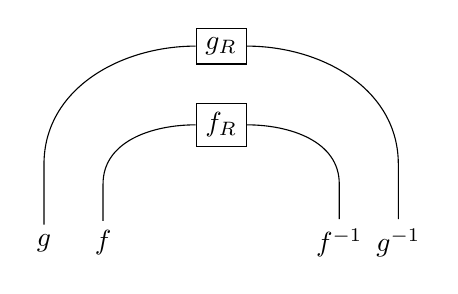
\begin{tikzpicture}
      \node[draw] (GR) {$g_R$};
      \node[on grid, below=1 of GR, draw] (FR) {$f_R$};
      \node[on grid, below left=1.5cm and 2.25cm of FR] (Base1) {$g$};
      \node[on grid, right=0.75cm of Base1] (Base2) {$f$};
      \node[on grid, right=3cm of Base2] (Base3) {$\inv f$};
      \node[on grid, right=0.75cm of Base3] (Base4) {$\inv g$};
      \draw (Base1) to ++(0,1cm) to [out=90,in=180]  (GR);
      \draw (Base4) to ++(0,1cm) to [out=90,in=0] (GR);
      \draw (Base2) to ++(0,0.75cm) to [out=90,in=180] (FR);
      \draw (Base3) to ++(0,0.75cm) to [out=90,in=0] (FR);
    \end{tikzpicture}
  \end{center}
\end{frame}

\begin{frame}
  \frametitle{Respecting the graphical calculus}
  \begin{theorem}
    In a 2-category, if two string diagrams are planar isotopic then the two morphisms they represent are equal.
  \end{theorem}
  \pause{}
  \begin{definition}
    An \(\omega\)-category \emph{respects the graphical calculus} if, for any pair of string diagrams with a planar isotopy between them, there is a quasi-invertible \(3\)-cell from the cell represented by the first to the cell represented by the second.
  \end{definition}
\end{frame}

\begin{frame}
  \frametitle{Properties of quasi-invertible structures}
  \begin{itemize}
  \item Given a quasi-invertible structure of \(f\), there exists a quasi-invertible structure on \(\inv f\).
  \item There is a quasi-invertible structure on any identity morphism.
  \end{itemize}
\end{frame}

\begin{frame}[fragile]
  \frametitle{Limitations of quasi-invertibility}
  Take the \(\omega\)-category generated by \(0\)-cells \(x\) and \(y\) and a quasi-invertible morphism \(f : x \to y\).

  \pause{}
    \begin{center}
    \begin{tikzpicture}
      \node (Bottom) {$f$};
      \node[on grid, above right=1cm and 2.25cm of Bottom, draw] (Cup) {$\inv {f_L}$};
      \node[on grid, above left=2cm and 1.5cm of Cup,draw] (Cap){$f_R$};
      \node[on grid, above right=1cm and 2.25cm of Cap] (Top) {$f$};
      \draw (Bottom) to++(0,2) to[out=90,in=180] (Cap);
      \draw (Cup) to[out=180,in=-90] ++(-0.75,1) to[out=90,in=0] (Cap);
      \draw (Cup) to[out=0,in=-90] ++(0.75,1) to (Top);
    \end{tikzpicture}
  \end{center}
\end{frame}


\begin{frame}
  \frametitle{Invertibility in type theory}
  Inverses of \(f : A \to B\):
  \begin{itemize}
  \item Quasi-invertible:
    \[ \mathsf{qinv}(f) : \Sigma_{g : B \to A} f \circ g \sim \id_B \times g \circ f \sim \id_A\]
  \item Bi-invertible:
    \begin{align*}
      &\mathsf{binv}(f) : \mathsf{linv}(f) \times \mathsf{rinv}(f) \\
      &\mathsf{linv}(f) : \Sigma_{g : B \to A} g \circ f \sim \id_A \\
      &\mathsf{rinv}(f) : \Sigma_{g : B \to A} f \circ f \sim \id_B
    \end{align*}
  \item Half-adjoint invertible:
    \[ \mathsf{ishai}(f) : \Sigma_{g : B \to A} \Sigma_{\eta : g \circ f \sim \id_A} \Sigma_{\epsilon : f \circ g \sim \id_B} \Pi_{x : A} f(\eta x) = \epsilon(f x) \]
  \end{itemize}
\end{frame}

\begin{frame}
  \frametitle{Bi-invertibility}
    Given an \(n\)-cell \(f : x \to y\), a \emph{bi-invertible} structure on \(f\) is a tuple \((\rinv f, \linv f, f_R, f_L, f_R{}BI, f_L{}BI)\) where:
  \begin{itemize}
  \item \(\rinv f\) is an \(n\)-cell \(y \to x\);
  \item \(\linv f\) is an \(n\)-cell \(y \to x\);
  \item \(f_R\) is an \((n+1)\)-cell \(f \comp_1 \rinv f \to \id_x\);
  \item \(f_L\) is an \((n+1)\)-cell \(\linv f \comp_1 f \to \id_y\).
  \item \(f_R{}BI\) is a bi-invertible structure on \(f_R\).
  \item \(f_L{}BI\) is a bi-invertible structure on \(f_L\).
  \end{itemize}
\end{frame}

\begin{frame}
  \frametitle{Properties of bi-invertible structures}
  \begin{itemize}
  \item Any quasi-invertible structure can be converted to a bi-invertible structure.
  \item Given a bi-invertible structures on a pair of compatible morphisms, there is a bi-invertible structure on their composite.
  \item Given a bi-invertible structure on \(f\), \(f, \rinv f, \linv f, \dots\) there are bi-invertible structures on both \(\rinv f\) and \(\linv f\).
  \end{itemize}
  \pause{}
  These are proved using coinduction and the results have been formalised in Agda using sized types.
\end{frame}

\begin{frame}[fragile]
  \frametitle{Half-adjoint invertibility}
  \begin{definition}
  Given an \(n\)-cell \(f : x \to y\), a \emph{half-adjoint invertible} structure on \(f\) is a tuple \((f', \alpha_f, \beta_f, \gamma_f, \alpha_f{}HAI, \beta_f{}HAI, \gamma_f{}HAI)\) where:
  \begin{itemize}
  \item \(f'\) is an \(n\)-cell \(y \to x\);
  \item \(\alpha_f\) is an \((n+1)\)-cell \(f \comp_1 f' \to \id_y\);
  \item \(\beta_f\) is an \((n+1)\)-cell \(\id_x \to f' \comp_1 f\);
  \item \(\gamma_f\) is an \((n+2)\)-cell \((\lambda_{f'}^{-1} \comp_1 (\beta_f \comp_2
 \id_{f'}) \comp_1 a_{f',f,f'} \comp_1 (\id_{f'} \comp_2 \alpha_f) \comp_1 \rho_{f'}) \to \id_{f'}\);
  \item \(\alpha_f{}HAI\) is a half-adjoint invertible structure on \(\alpha_f\);
  \item \(\beta_f{}HAI\) is a half-adjoint invertible structure on \(\beta_f\);
  \item \(\gamma_f{}HAI\) is a half-adjoint invertible structure on \(\gamma_f\).
  \end{itemize}
  \end{definition}
\end{frame}

\begin{frame}
  \frametitle{Half-adjoint invertibility}
  \begin{center}
    \begin{tikzpicture}
      \node (Bottom) {\({f'}\)};
      \node[on grid, above left=1cm and 2.25cm of Bottom, draw] (Cup){\(\beta_f\)};
      \node[on grid, above right=2cm and 1.5cm of Cup,draw] (Cap){\(\alpha_f\)};
      \node[on grid, above left=1cm and 2.25cm of Cap] (Top) {\({f'}\)};
      \draw (Bottom) to++(0,2) to[out=90,in=0] (Cap);
      \draw (Cup) to[out=0,in=-90] ++(0.75,1) to[out=90,in=180] (Cap);
      \draw (Cup) to[out=180,in=-90] ++(-0.75,1) to (Top);

      \node[on grid, above right=2cm and 1cm of Bottom, font=\fontsize{20}{24}\selectfont] (Eq) {\(\Rightarrow\)};
      \node[above=0cm of Eq,font=\fontsize{15}{19}\selectfont] (Gamma) {\(\gamma_f\)};
      \node[on grid, right=2cm of Bottom] (L1) {\({f'}\)};
      \node[on grid, above=4cm of L1] (L2) {\({f'}\)};
      \draw (L1) to (L2);
    \end{tikzpicture}
  \end{center}
\end{frame}

\begin{frame}
  \frametitle{Adjoint equivalence}
  \begin{definition}
    A \emph{adjoint equivalence} between categories \(\mathcal C\) and \(\mathcal D\) is an equivalence \((F,G,\eta,\epsilon)\) such that \(F \dashv G\) with unit \(\eta\) and counit \(\epsilon\)
  \end{definition}

  \pause{}
  An adjoint equivalence is precisely a half-adjoint invertible structure in \textbf{Cat}.
\end{frame}

\begin{frame}
  \frametitle{Main theorem}

  \begin{theorem}
  Let \(G\) be a globular set with the given higher category properties. Let \(n > 0\) and \(f\) be an \(n\)-cell of \(G\). Then the following are equivalent:
  \begin{itemize}
  \item \(f\) has a bi-invertible structure.
  \item \(f\) has a quasi-invertible structure.
  \item \(f\) has a half-adjoint invertible structure.
  \end{itemize}
\end{theorem}
\end{frame}

\begin{frame}
  \frametitle{Further work}
  \begin{itemize}
  \item A limitation of quasi-invertible structures was presented earlier. Do bi-invertible structures and half-adjoint invertible structures have the same limitation?
  \item The ``respects the graphical calculus'' condition is slightly mysterious. It would be good to find a set of more concrete conditions from which it follows.
  \item Can coinduction be used to nicely describe other parts of higher category theory?
  \end{itemize}
\end{frame}

\begin{frame}
  \frametitle{Bi-invertibility implies half-adjoint invertibility}
\end{frame}

\end{document}